%!TEX encoding = UTF-8 Unicode
\section{Requisitos Funcionais}
\hspace{15pt}A nossa solução é modular afim permitir a combinação de funcionalidades e a rápida extensabilidade. A Figura\ref{fig:arch} explicita a arquitectura da nossa solução. Consultamos vários sites de feeds, extraimos os links para a notícia original, descarregamos a noticia, extraimos as entidades presentes e analisamos o sentimento de cada uma das frases da noticia e associamos esse sentimento à entidade de cada frase. Em todos os casos a informação é guardada em varias tabelas utilizando uma base de dados local \textbf{(sqlite3)}. As tabelas foram desenhadas por foram a poderemos efectuar pesquisas eficientes e complexas sobrea a base de dados. A linguagem de programação utilizada foi o \textbf{Python}. Utilizamos tambem algumas faramentas para processar e indexar a informação como é o caso do \textbf{Whoosh}, o \textbf{Feedparser}, o \textbf{Beautiful Soup} e o \textbf{NTLK}.
\begin{figure}[ht!]
\centering
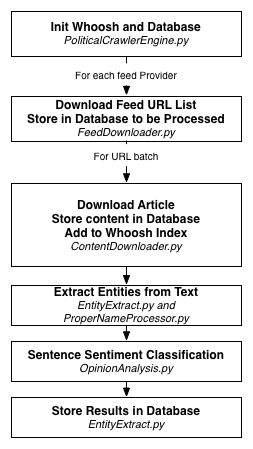
\includegraphics[width=0.42\textwidth]{./Figures/arch}
\caption{Arquitectura do Sistema}
\label{fig:arch}
\end{figure}
